\documentclass[a4paper,10pt]{article}
\usepackage[utf8]{inputenc}
 
% Blank line between paragraphs instead of indenting the first line
\usepackage{parskip}
\setlength{\parskip}{\baselineskip}

% Squash a bit more text onto a page
\usepackage{geometry}
\geometry{verbose,tmargin=20mm,bmargin=20mm,lmargin=25mm,rmargin=25mm}

\usepackage{graphicx}
\usepackage{listings}
\usepackage{amsmath}
\usepackage{verbatim}
\usepackage{xcolor}
\usepackage{dirtree}

% Indent verbatim environments
\makeatletter \def\verbatim@processline{\hspace*{2em}\the\verbatim@line\par}\makeatother

\lstdefinelanguage{logicdef}
{
  morekeywords={DEVICES, MONITORS, CONNECTIONS, END},
  sensitive=false,
  morecomment=[s]{/*}{*/},
  basicstyle=\small\ttfamily,
  keywordstyle=\pmb,
  frame=single,
  numbers=left,
  numberstyle=\tiny
}

\definecolor{darkgreen}{rgb}{0,0.7,0}
\definecolor{darkred}{rgb}{0.7,0,0}

\lstdefinelanguage{diff}
{
  morecomment=[f][\color{blue}]{@@},     % group identifier
  morecomment=[f][\color{darkred}]{-},         % deleted lines 
  morecomment=[f][\color{darkgreen}]{+},       % added lines
  morecomment=[f][\color{magenta}]{---}, % Diff header lines (must appear after +,-)
  morecomment=[f][\color{magenta}]{+++},
  basicstyle=\small\ttfamily,
  breakatwhitespace=false,         % sets if automatic breaks should only happen at whitespace
  breaklines=true,                 % sets automatic line breaking
  frame=single,
  numbers=none
}

\definecolor{mygreen}{rgb}{0,0.6,0}
\definecolor{mygray}{rgb}{0.5,0.5,0.5}
\definecolor{mymauve}{rgb}{0.58,0,0.82}

\lstset { 
  backgroundcolor=\color{white},   % choose the background color; you must add \usepackage{color} or \usepackage{xcolor}
  basicstyle=\small\ttfamily,      % the size of the fonts that are used for the code
  breakatwhitespace=false,         % sets if automatic breaks should only happen at whitespace
  breaklines=true,                 % sets automatic line breaking
  captionpos=b,                    % sets the caption-position to bottom
  commentstyle=\color{mygreen},    % comment style
  deletekeywords={...},            % if you want to delete keywords from the given language
  escapeinside={\%*}{*)},          % if you want to add LaTeX within your code
  extendedchars=true,              % lets you use non-ASCII characters; for 8-bits encodings only, does not work with UTF-8
  frame=single,                    % adds a frame around the code
  keepspaces=true,                 % keeps spaces in text, useful for keeping indentation of code (possibly needs columns=flexible)
  columns=flexible,
  keywordstyle=\color{blue},       % keyword style
  language=C++,                    % the language of the code
  morekeywords={*,DEVICES,
  				CONNECTIONS,
  				MONITORS,
  				END}, 	           % if you want to add more keywords to the set
  numbers=left,                    % where to put the line-numbers; possible values are (none, left, right)
  numbersep=5pt,                   % how far the line-numbers are from the code
  numberstyle=\tiny\color{mygray}, % the style that is used for the line-numbers
  rulecolor=\color{black},         % if not set, the frame-color may be changed on line-breaks within not-black text (e.g. comments (green here))
  showspaces=false,                % show spaces everywhere adding particular underscores; it overrides 'showstringspaces'
  showstringspaces=false,          % underline spaces within strings only
  showtabs=false,                  % show tabs within strings adding particular underscores
  stepnumber=1,                    % the step between two line-numbers. If it's 1, each line will be numbered
  stringstyle=\color{mymauve},     % string literal style
  tabsize=2,                       % sets default tabsize to 2 spaces
  title=\lstname                   % show the filename of files included with \lstinputlisting; also try caption instead of title
}

\begin{document}

\begin{center}
\LARGE \textbf{IIA GF2 Software: Final Report}

Martin Jackson (mj380) - Churchill College\\
Team 8
\end{center}

\tableofcontents{}\pagebreak

\section{Software function}
%%% Brief description of the function of the logic simulator
This software project involved completing the development of a logic simulation program, and subsequently performing maintenance on it. The finished program is capable of simulating a circuit containing any number of connected:
\begin{itemize}
\item Clocks, which change state every \texttt{n} cycles, where \texttt{n} can be configured separately for each clock and can be any number greater than zero.
\item Switches, which can be changed by the user during simulation.
\item AND, NAND, OR, NOR logic gates, with 1 to 16 inputs.
\item XOR gates, with two inputs.
\item D-type flip flops, with the normal data, clock, set and reset inputs, and normal and inverted outputs.
\item Signal generators, which produce an arbitrary periodic binary waveform of any length.
\end{itemize}

The simulator can read a circuit from a file (in plain text, extension \texttt{.gf2}, syntax as described in appendix~\ref{sec:EBNF}), simulate it, and display signal traces recorded during simulation. In addition, circuits can be edited from within the GUI. Instructions on how to use the program are given in appendix~\ref{sec:guide}. Example circuits are given in appendix~\ref{sec:examples}.

\section{Teamwork}
%%% Short commentary on the approach taken to teamwork
The team operated in a flexible manner. Though tasks were initially assigned to each team member, and each team member worked mainly on their assigned areas of the code, we assisted each other where necessary. I worked mainly on the GUI, but also wrote automated tests for the scanner and names classes, and helped out the other members of my team with any difficulties they encountered. 

\texttt{git}+GitHub were used for version control, with over 250 commits made during the course of the project. Using \texttt{git} allowed us to work independently, with minimal time wasted on source code management and synchronising and merging changes. It was also extremely helpful in allowing more than one person to work on the same part of the program simultaneously, when this was necessary in order to complete tasks on time, or to allow other team members to help track down and fix complex bugs.

Github was used for bug tracking, though this was mainly for bugs that needed to be communicated to the rest of the team - any bugs we found in our own areas of the code we just fixed immediately.

Overall, the team worked well together, meeting all deadlines and producing a working program which we believe adequately meets the client's specifications. 

\subsection{Development phase}
Areas of development were initially allocated as shown in the Gantt chart in the first report. I worked on the GUI, Jamie on the names and scanner classes, and Tim on the parser class. 

Integration of modules was done as early as possible. The main \texttt{logsim} program was first compiled with a ``File $\rightarrow$ Open'' command that called the parser and scanner modules on 20th May (when these modules contained no code, just an outline of the interface). The GUI at this stage also had a textbox that displayed all messages printed to \texttt{cout}. Integration of the GUI with the scanner and parser modules could then be tested using the main \texttt{logsim} program as soon as those modules were written. GUI development was performed almost entirely with the main \texttt{logsim} program, instead of using the supplied \texttt{guitest} program. 

I completed the core functionality for the GUI on 27th May, as scheduled in the Gantt chart. The remaining time before the second interim report was scheduled for integration and final testing. However, since the modules had already been integrated and there were no problems visible in the GUI, and I was therefore ahead of schedule, I used this time to add the ability to edit device properties and connections to the GUI. Meanwhile, Tim and Jamie finished the parser and performed final testing. 

\subsection{Maintenance phase}
We split the maintenance work between us, with one task per person.

I implemented the continuous simulation feature. However, since I had already implemented most of the functionality before the maintenance phase (by adding a scrollable signal traces display, and allowing an unlimited number of monitor samples), I was able to complete the task very quickly by just adding a timer and a button. 

I was therefore able to make some enhancements to the GUI during the maintenance phase, and assist Jamie with the D-type bistable changes. Tim added the signal generator and made improvements to the parser. 

\section{Software}
%%% Brief description of the software structure
%%% Brief description of the software written and/or modified by you
This section contains a description of the general software structure. Some more detailed notes on the parts of the software written or modified by me are also included. I was responsible for the GUI, and for most of the changes to the supplied source code (the devices, network, and monitors classes). 

\subsection{Circuit classes}
The \texttt{network} class is used for storing and searching the list of devices, for managing connections between devices, and to handle allocation of memory for devices. The \texttt{devices} class handles creation of individual devices and simulation of the circuit. I added several functions to these class to assist with device editing from the GUI, Tim added functions for the signal generator, Jamie made a function in the network class to sort the device list randomly, and Jamie and I jointly modified the D-type bistable code. 

The \texttt{monitors} class is used to contain monitor data, and has functions for adding and removing monitors, and logging the current state of all monitored outputs. I modified this class to remove the limit on the number of samples and monitors, by using STL vectors. 

The \texttt{names} class is used by all other classes to handle conversion between strings and the internal representation of strings. For efficiency, strings are represented internally in the logic simulator as integers. 

\subsection{File loading}
Three classes are involved in loading a file. The \texttt{scanner} class transforms the characters in the input file into symbols for the parser, stripping out unnecessary things like comments and whitespace. The \texttt{parser} class calls the scanner class to obtain symbols, and checks that the symbol sequence conforms to the EBNF syntax and satisifes all semantic rules. It then calls appropriate functions in the circuit classes to create the devices, connections, and monitors specified in the definition file. The \texttt{error} class is called by the parser whenever it encounters an error, and is responsible for counting errors and warnings and printing out error and warning messages. 

\subsection{GUI - circuit interface}
Since a lot of the GUI needs to make use of many of the circuit simulation classes, and these classes need to be recreated and pointers updated when loading a file, I created a new class named \texttt{circuit} to contain these pointers and pass them around between GUI classes. The observer pattern was used to notify all necessary GUI components of changes to the devices in the circuit, the monitors, and the number of monitor samples. 

\subsection{GUI - main frame}
The main window is defined in \texttt{gui.cc}. This is the core of the application, creating all other controls and windows, and constructing the main instance of the \texttt{circuit} class. 

\subsection{GUI - canvas}
Monitor traces are scaled to fit the window, with appropriate limits on how much they can be scaled by. Cycle numbers are drawn at appropriate intervals, with the interval changing according to the signal trace scale, and lying in the set $10^n \times \{1, 2, 5\}$ for $n \geq 0$.

The display of each monitor trace within the canvas is handled by a separate class, GLCanvasMonitorTrace. MyGLCanvas constructs a new instance of GLCanvasMonitorTrace for each monitor when the number of monitors changes. 

Some things that I encountered that it may be useful to look into for future years:
\begin{itemize}
 \item Calling the MyGLCanvas::Render() function directly can sometimes cause a crash. A safer alternative is to use Refresh() and Update() calls to queue a paint event instead. 
 \item I needed to use the following sequence of calls to guarantee that the canvas was redrawn correctly: ``Refresh(); Update(); Refresh();''. This was most noticeable while testing a cross-compiled executable in Wine after implementing canvas scrolling. Before using these calls, the canvas did not always update after scrolling. Another team consulted me after experiencing similar symptoms with their canvas, and using this sequence of calls seemed to fix it for them too. These calls may or may not all be needed if the canvas does not scroll, I have not tested it.
\end{itemize}

\subsection{GUI - scrolling canvas}
Since making the scrolling monitor traces canvas work well took a little digging through the wxWidgets source code, and the solution may not be obvious, some explanation is merited. 

The naive solution is to make MyGLCanvas large enough to fit all the monitors and samples, and place it as a child inside a wxScrolledWindow. This was the strategy that I tried first. However, this is quite laggy when the canvas size is large, and suffers from some artifacts during scrolling. 

I therefore used a different strategy. I made the MyGLCanvas class inherit from both wxGLCanvas and wxScrollHelperNative. wxScrollHelperNative is the class that wxScrolledWindow inherits from - a helpful inheritance diagram and some comments can be found in the wxWidgets \texttt{wx/scrolwin.h} header file. wxScrollHelperNative is a mix-in class which manages scroll bar visibility, position and size for a control or window, based on the size of the scrolled area set with SetVirtualSize. 

MyGLCanvas was then modified to implement its own scrolling. ScrollWindow, the function that wxScrollHelperNative calls in response to scrollbar movement in order to actually move the contents of the scrolled area, was overridden. The ScrollWindow function in MyGLCanvas modifies some member variables and requests a redraw of the canvas. The positions of the drawn monitor traces are then offset according to these member variables. The canvas and drawing area remain the same size and in the same position, it is only the virtual size and the positions of drawn points on the canvas which change. 

When the canvas is resized or the number of monitors or recorded samples changes, the MyGLCanvas class updates its virtual size to be the minimum area needed to display them all, based on the minimum trace scaling factors.

In addition, to prevent lag when a large number of samples have been recorded, only those samples within the visible area will be fetched from the monitor class and drawn. 

\subsection{GUI - device editing}

%% TODO

\subsection{Circuit simulation modifications}
For the D-type flip flop maintenance modifications, our initial strategy to prevent the result of simulation depending on the order in which devices were declared in the definition file was to sort the list of devices in the network class randomly. However, this made testing difficult, as the randomised device order affected logic gate propagation delays (used to delay the clock and data inputs by different amounts when testing the D-type changes), which made the offset between clock and data inputs randomly vary. 

A better solution to the device declaration order problem is to double buffer changes to output signals. This means that changes to output signals are visible to other devices only during the next machine cycle, and never during the same machine cycle that the changes are made in. The \texttt{signalupdate()} function stores the new output signal in a new variable \texttt{nextsig}, and this is copied into \texttt{sig} at the end of every machine cycle. This completely eliminates all effects of device declaration order on circuit behaviour. 

D-type flip flops were modified to check for rising/falling edges in the input immediately before, during, and immediately after the rising clock edge, and the output will be random if a rising or falling edge occurs in any of these three machine cycles. An option was added to the GUI to print warnings when a D-type output is indeterminate.

The randomised device order was left in the simulator after the double buffering was added, as a demonstration that behaviour no longer depends on device order. 

\section{Test procedures}
%%% Description of the test procedures adopted

For the names and scanner classes, I wrote automated unit tests which compared the results from various functions to expected results. The source code for these was included in my second interim report in appendix~\ref{sec:report2}. Some of the tests were written before the code to be tested was written, and some modified or added afterwards to target potential problems that I spotted (essentially, peer review of the code). The process of fixing problems, and adding tests to look for new problems was iterated several times. 

For the parser, continuous integration testing was used. The thorough unit tests for the scanner and names classes meant that the parser could be tested using a set of example circuit definition files, with reasonable confidence that any problems originated from the parser rather than the scanner or names classes. The working example definition files were used, along with a set of files with errors deliberately introduced to test the various error messages and error handling. A shell script was later written by Jamie to automatically load all these definition files and log the output. 

Since this was the first time that I have used wxWidgets, the GUI software structure and functionality was mostly designed on the fly whilst I explored the capabilities of wxWidgets (though sketches of the desired GUI appearance were made before development was started). This, combined with the non-trivial work involved in making automated tests for a GUI, meant that no unit tests were produced for the GUI, and only manual system testing was used. 

Usability testing was performed by observing the actions of the demonstrator during the software testing for the second interim report. Usability enhancements based on these observations and feedback from the demonstrator were implemented during the maintenance phase (for example, a menu item to reload the current file, and remembering the selected directory between invocations of the open file dialog). 

For most tests, best practice was followed by having different people write the tests and the code to be tested. Jamie implemented the scanner and names classes, and I wrote tests for them. Tim was responsible for most of the parser class, and Jamie created most of the circuit definition files to test individual error messages in the parser.  

The changes to D-type flip-flops were testing during implementation by printing various debugging messages to the log textbox when the output of the D-type was indeterminate. Circuits where the input signal changed before, during, and after the rising clock edge were created by adding logic gates before the D-type clock or data inputs to introduce a delay in signal propagation.

While Jamie was implementing changes in the devices and network classes, I added a feature to the GUI which allows the internal function of the logic simulator to be visualised, showing the times at which different signals rise or fall relative to each other. Some of the debugging messages used when testing the changes were left in the code, and an option added to the GUI to enable these warnings, notifying the user when the output of a D-type is indeterminate. 

As an example, the visualisation of internal circuit function for a circuit where the input changes during clock rise, setup time, or hold time for each of three D-type bistables is shown in figure~\ref{fig:dtype-each}. The warnings generated are:

\begin{verbatim}
 Warning: indeterminate output for D-type D3, input changed during clock rise
 Warning: indeterminate output for D-type D1, input changed during setup time
 Warning: indeterminate output for D-type D2, input changed during hold time
\end{verbatim}

\begin{figure}[h]
 \centering
 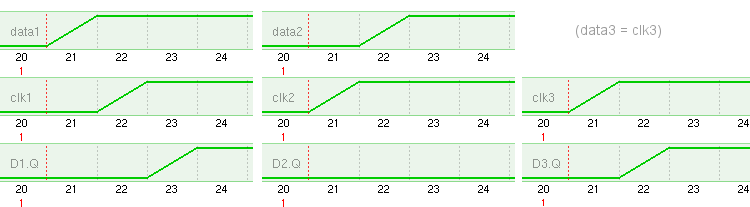
\includegraphics[width=16cm]{dtype-test2.png}
 \caption{Internal logic simulator function shown for D-types where the data signal changes around the time of the rising clock edge. The dashed line just to the right of the monitor name signifies the start of the simulation cycle. Each cycle shown after that dashed line is one \texttt{machinecycle}, corresponding to one internal step of the simulation.}
 \label{fig:dtype-each}
\end{figure}

The resulting outputs are random. Circuits with the input change outside three machine cycles centred on the rising clock edge were also tested to confirm that the D-type modifications were operating correctly. In those cases, the output was not random, and was less interesting so is not included in this report. 

\section{Recommendations for improvement}
%%% Conclusions and recommendations for improvement
I believe that the client's requirements have been fulfilled. Some extra features not requested by the client have also been added. However, there are some additional ideas that I've had, and some things that other team members have suggested, which could have been implemented if there was time. These include:

\begin{enumerate}
 \item Exporting monitor traces as a CSV file
 \item Printing monitor traces, or saving them as an image.
 \item Add more devices.
 \item Improved simulation of circuit timing, such as gate propagation delays. As an extension to this, perhaps some way of alerting the user to logic hazards. 
 \item Generation of a circuit from a boolean algebra expression.
 \item A way of resetting all switch states to the initial values in the circuit definition file, without reloading the whole circuit and resetting all other component states in the process.
 \item Ability to reorder monitors, perhaps by dragging and dropping them in the traces display.
 \item Saving the circuit to a file. This would allow new circuits to be created from within the GUI, or modifications to existing circuits to be changed.
 \item Compatibility with files from other logic simulation programs (limited to devices that exist within this logic simulator).
\end{enumerate}


\section{Conclusions}
Though there are areas where the logic simulator could be improved, we believe that the client's requirements have been met. The thorough testing ensured that almost all parts of the logic simulator worked well. Almost all required functionality was complete in time for each deadline. Use of \texttt{git} for version control was extremely useful for tracking and merging changes, and played a key part in allowing the team to collaborate efficiently. 

\appendix

\section{Example Definition Files}
\label{sec:examples}
Example definition files for functionality that existed prior to the maintenance phase can be found in the second interim report in appendix~\ref{sec:report2}. Only the additional files for functionality added in the maintenance phase of the project are shown below. 

\subsection{Signal Generator Example}

\subsubsection{Definition File}
\lstinputlisting[caption=siggen.gf2]{../../examples/siggen.gf2}

\subsubsection{Circuit Diagram}
\begin{figure}[h]
 \centering
 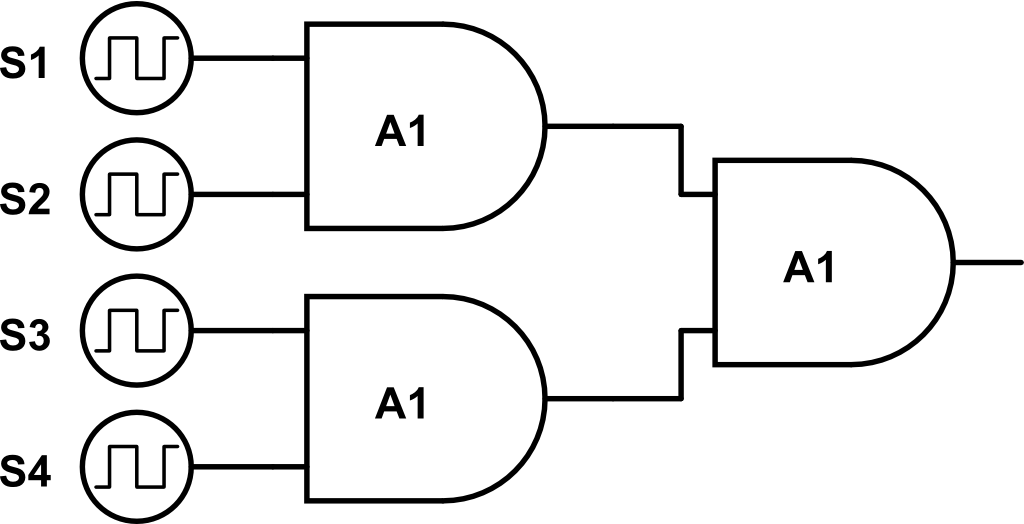
\includegraphics[width=9cm]{../../examples/siggen.png}
 \caption{Circuit diagram using a signal generator}
 \label{fig:example-siggen}
\end{figure}

\textbf{NB} The software used to draw the circuit diagram does not support the AND gates with four inputs. Therefore three AND gates with two inputs each were substituted for the single AND gate, A1, with four inputs as can be seen in Fig. \ref{fig:example-siggen}.



\section{EBNF}
\label{sec:EBNF}
\lstinputlisting[caption=EBNF, language=python]{../../docs/ebnf.txt} %python seems to work okay


\clearpage
\section{User Guide}
\label{sec:guide}
\textbf{Opening files.} There are two methods of opening a file. Either pass the filename as a command line argument when starting the logic simulator, or use the ``File $\rightarrow$ Open'' menu item and select the correct file. Logic circuit definition files are plain text files with extension \texttt{.gf2}. Examples are provided in section~\ref{sec:examples}. Any errors which occur while loading the file will be shown in the textbox at the bottom of the window.

\textbf{Running the simulation.} After opening a circuit, select the number of cycles to simulate using the textbox in the top right corner. Then click the ``Run'' button just below the textbox. Results will be displayed in the large space to the left. The run button clears the displayed results and simulates the circuit for the specified number of cycles. To simulate for additional cycles without clearing the displayed results, use the ``Continue'' button instead. The only limit on the number of displayed signals and simulated cycles is the available memory on the computer.  If necessary, scrollbars will appear around the result display area. 

\textbf{Running continuously.} The ``Run continuously'' button can be used for indefinite, continuous simulation, with signal traces scrolling (in the manner of an oscilloscope) until stopped. The rate of simulation is adjustable in the options dialog, accessible from the options menu, and can also be changed using keyboard shortcuts as displayed in the options menu. 

\textbf{Adding or removing monitors.} To change which signals are monitored and displayed, use the add or remove monitors buttons on the right. The add monitors button will show a list of unmonitored outputs that can be selected for monitoring, and the remove monitors button a list of current monitors that can be removed. In both cases, multiple items may be selected. After adding a monitor, you must use the run button before using the continue button, as no samples were recorded for the new monitor during the cycles displayed on screen, so the recorded signals cannot be continued, they must be reset first. 

\textbf{Changing switch states.} Use the checkboxes located in the bottom right corner of the window. Changes take effect immediately. Run or continue the simulation to see the effect on the circuit. 

\textbf{Editing devices.} Click the edit devices button on the right hand side. This will open a window allowing you to add, edit, or delete devices. Select a device to edit using the list on the left. The top panel allows device properties to be modified. The bottom panels show inputs and outputs for the selected device, and which devices are connected to it. They also allow connections to be added and deleted. All changes to devices and connections take effect immediately, except for changes to device properties, which must be confirmed using the ``Apply changes'' button. 

\textbf{D-type bistable model.} The D-type bistable model incorporates non-zero setup and hold times. In the options dialog, there is a debug option that will cause warnings to be printed when the input changes during these times, and also an option to display the state of monitored signals during each step used internally in a simulation cycle (called a \texttt{machinecycle}, with all gate propagation delays being at least one \texttt{machinecycle} long). These options will help you find and fix changes in input during setup and hold times. Setup and hold times are one \texttt{machinecycle} either side of the \texttt{machinecycle} containing the rising clock edge, and a random output will be produced if the input rises or falls during setup or hold times, or during the rising clock edge. 

\clearpage
\section{File Listing}

%%To install dirtree for your account in the Engineering department:
%mkdir -p ~/texmf/tex/latex/dirtree
%cd ~/texmf/tex/latex/dirtree
%wget http://mirrors.ctan.org/macros/generic/dirtree/dirtree.dtx
%wget http://mirrors.ctan.org/macros/generic/dirtree/dirtree.ins
%latex dirtree.ins

\setlength{\DTbaselineskip}{15pt}
\DTsetlength{.2em}{3em}{0.1em}{1pt}{4pt}
\dirtree{.1 logsim.
.2 docs.
.2 examples.
.3 errors.
.2 report1.
.2 report2.
.2 report3.
.2 src.
.3 names.*.
.3 scanner.*.
.3 parser.*.
.3 error.*.
.3 devices.*.
.3 network.*.
.3 monitor.*.
.3 gui.*.
.3 logsim.*.
}

\textbf{docs} contains documentation relevant to our logic simulator such as: EBNF, reserved words, and our Gantt chart.

\textbf{examples} contains our example definition files as listed in Appendix~\ref{sec:examples} as well as the shell script written by Jamie to open each example definition file in the logic simulator and log the output for testing purposes.

\textbf{errors} contains definition files which contain deliberate errors and are used to test our error checking functionality. In addition this folder contains the error.sh shell script written by Jamie to open each erroneous definition file in the logic simulator and log the output for testing purposes.

\textbf{report1, report2} and \textbf{report3} contain our first, second and final report respectively.

\textbf{src} contains the source code for our logic simulator. The functionality of the major classes is outlined beneath.

\textbf{names} stores a list of all the words used within a definition file, and methods to manipulate them. It is initialised with only the reserved words, but can be populated as a definition file is read.

\textbf{scanner} reads through the definition file, character by character, and is able to return complete symbols to the parser. It is able to return the internal representation of a symbol, the type of symbol and optionally the value.

\textbf{parser} analyses the definition file as it is read in according to the rules laid out in our EBNF. It is then able to create devices, connections and monitors that are laid out in the definition file.

\textbf{error} is used by the parser to count errors and warnings and print the error and warning messages. 

\textbf{devices} is used to create and execute devices. 

\textbf{network} stores information about the devices, including the connections between each device.

\textbf{monitor} implements signal monitors, which are used to display the points of interest, as determined from the definition file, in the GUI.

\textbf{gui} files provide a graphical user interface for the user, and allow for advanced features such as circuit and monitor editing without having to edit the definition file. The GUI classes are split into several files according to function. 

\begin{itemize}
 \item \textbf{gui} contains the main window, and the dialogs for adding or removing monitors.
 \item \textbf{gui-canvas} is the canvas for displaying signal traces.
 \item \textbf{gui-devices} is the device editing dialog, and the dialogs for creating new devices or connections that are used by the device editing dialog.
 \item \textbf{gui-devices-infopanels} contains the panels used for displaying information in the device editing dialog. A panel contains either device details, or information about all inputs to a device, or details of a single output.
 \item \textbf{gui-id} defines unique identifiers for all controls that need a unique identifier.
 \item \textbf{gui-misc} contains miscellaneous widgets and GUI functions.
 \item \textbf{gui-options} is the dialog for changing simulation options, and the class that contains the current option values.
\end{itemize}

\textbf{logsim} ties all the other classes together and allows the user to fully simulate logic circuits.


\clearpage
\section{Source code before maintenance modifications}
\label{sec:report2}

A complete listing of all source code written by me, not including modifications made during the maintenance phase, can be found in my second interim report (attached).

\end{document}

